\documentclass{beamer}
\usepackage[utf8]{inputenc}
\usetheme{Warsaw}
\usepackage[french]{babel}

\title{Projet C\\---\\Commutateur niveau 3}
\author{Philippe \bsc{Tran Ba} - Élie \bsc{Bouttier} - Jiajun \bsc{Shi} - Émilie \bsc{Abia}}
\institute{ENSEEIHT, département TR}

\usepackage{xcolor,times}


% Faire apparaître un sommaire avant chaque section
\AtBeginSection[]{
   \begin{frame}
   \begin{center}{\Large Plan }\end{center}
   %%% affiche en début de chaque section, les noms de sections et
   %%% noms de sous-sections de la section en cours.
   %\tableofcontents[currentsection,hideothersubsections]
   \tableofcontents[currentsection,hideallsubsections]
   \end{frame} 
}

\usepackage{listings}
  \newcommand*\styleC{\fontsize{9}{10pt}\usefont{T1}{ptm}{m}{n}\selectfont }
  \newcommand*\styleD{\fontsize{9}{10pt}\usefont{OT1}{pag}{m}{n}\selectfont }

  \makeatletter
  % on fixe le langage utilisé
  \lstset{language=C}
  \edef\Motscle{emph={\lst@keywords}}
  \expandafter\lstset\expandafter{%
    \Motscle}
  \makeatother


  \definecolor{Ggris}{rgb}{0.45,0.48,0.45}

  \lstset{emphstyle=\rmfamily\color{blue}, % les mots réservés de matlab en bleu
  basicstyle=\styleC,
  keywordstyle=\ttfamily,
  commentstyle=\color{Ggris}\styleD, % commentaire en gris
  numberstyle=\tiny\color{red},
  numbers=left,
  numbersep=10pt,
  lineskip=0.7pt,
  showstringspaces=false}
  %  % inclure le fichier source
  \newcommand{\FSource}[1]{%
  \lstinputlisting[texcl=true]{#1}
  }


\newenvironment{changemargin}[2]{%
 \begin{list}{}{%
 \setlength{\topsep}{0pt}%
 \setlength{\leftmargin}{#1}%
 \setlength{\rightmargin}{#2}%
 \setlength{\listparindent}{\parindent}%
 \setlength{\itemindent}{\parindent}%
 \setlength{\parsep}{\parskip}%
 }%
 \item[]}{\end{list}}


  %\usepackage{test}

\begin{document}

\begin{frame}
\titlepage
\end{frame}

\begin{frame}
\tableofcontents
\end{frame}

\section{Introduction}

\section{Architecture du programme}

\begin{frame}[plain]
%\begin{center}
%\hspace{-1cm}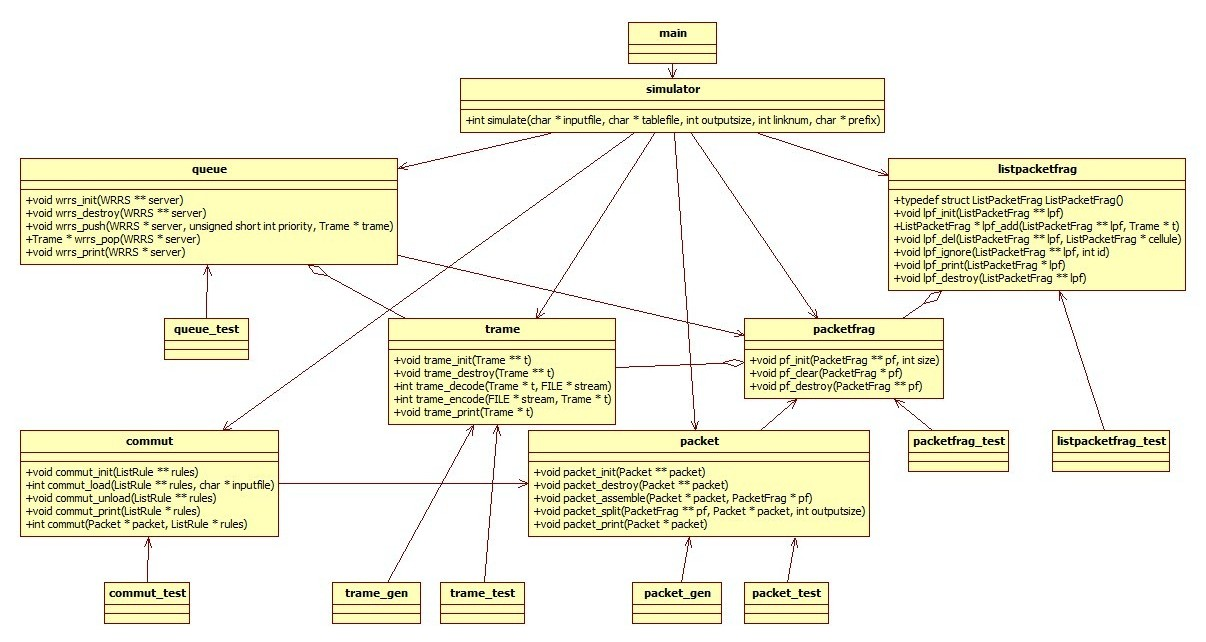
\includegraphics[scale=0.28]{UML2.jpg}
%\maxFrameImage{UML2.jpg}
%\end{center}
    \begin{changemargin}{-1cm}{-1cm}
        \begin{center}
            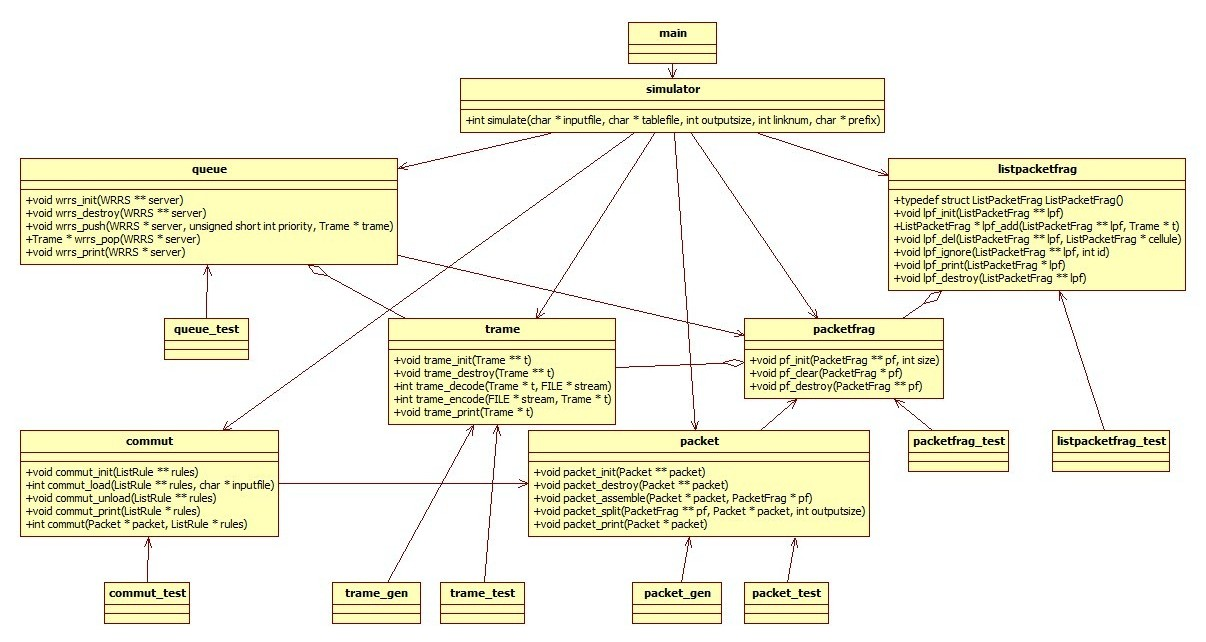
\includegraphics[width=\paperwidth,height=\paperheight,keepaspectratio]{UML2.jpg}
        \end{center}
    \end{changemargin}
\end{frame}

\frame{\center{\hspace{1.6cm}\includegraphics[scale=0.6]{s2.png}}}

\section{Implémentation}

\subsection{Trame}

\frame{\FSource{sources/trame.h}}

\frame{\FSource{sources/automate.c}}

\subsection{PacketFrag}

\frame{\FSource{sources/packetfrag.h}}

\subsection{ListPacketFrag}

\frame{\FSource{sources/listpacketfrag.h}}

\subsection{Packet}

\frame{\FSource{sources/packet.h}}

\subsection{Commut}

\frame{\FSource{sources/commut.h}}

\subsection{Queue}

\frame{\FSource{sources/queue.h}}

%\subsection{Main}

%\frame{\FSource{sources/main.c}}

\subsection{Simulator}

\frame{\FSource{sources/simulator.c}}
\frame{\FSource{sources/in.c}}
\frame{\FSource{sources/out.c}}

\section{Difficultées et améliorations}

\subsection{Difficultées}

\begin{frame}
    \begin{itemize}
        \item Lecture et « décodage à la volé » des trames
        \item Liste de liste de trame
        \item Ignorer les paquets dont la première trame reçu est erronée
        \item Calcul de la CRC
    \end{itemize}
\end{frame}

\subsection{Améliorations}

\begin{frame}
    \begin{itemize}
        \item Gestion des erreurs
        \item Asynchronisation des entrées/sorties
    \end{itemize}
\end{frame}

\section{Conclusion}

\end{document}
